\documentclass[twoside]{book}

% Packages required by doxygen
\usepackage{fixltx2e}
\usepackage{calc}
\usepackage{doxygen}
\usepackage[export]{adjustbox} % also loads graphicx
\usepackage{graphicx}
\usepackage[utf8]{inputenc}
\usepackage{makeidx}
\usepackage{multicol}
\usepackage{multirow}
\PassOptionsToPackage{warn}{textcomp}
\usepackage{textcomp}
\usepackage[nointegrals]{wasysym}
\usepackage[table]{xcolor}

% Font selection
\usepackage[T1]{fontenc}
\usepackage[scaled=.90]{helvet}
\usepackage{courier}
\usepackage{amssymb}
\usepackage{sectsty}
\renewcommand{\familydefault}{\sfdefault}
\allsectionsfont{%
  \fontseries{bc}\selectfont%
  \color{darkgray}%
}
\renewcommand{\DoxyLabelFont}{%
  \fontseries{bc}\selectfont%
  \color{darkgray}%
}
\newcommand{\+}{\discretionary{\mbox{\scriptsize$\hookleftarrow$}}{}{}}

% Page & text layout
\usepackage{geometry}
\geometry{%
  a4paper,%
  top=2.5cm,%
  bottom=2.5cm,%
  left=2.5cm,%
  right=2.5cm%
}
\tolerance=750
\hfuzz=15pt
\hbadness=750
\setlength{\emergencystretch}{15pt}
\setlength{\parindent}{0cm}
\setlength{\parskip}{0.2cm}
\makeatletter
\renewcommand{\paragraph}{%
  \@startsection{paragraph}{4}{0ex}{-1.0ex}{1.0ex}{%
    \normalfont\normalsize\bfseries\SS@parafont%
  }%
}
\renewcommand{\subparagraph}{%
  \@startsection{subparagraph}{5}{0ex}{-1.0ex}{1.0ex}{%
    \normalfont\normalsize\bfseries\SS@subparafont%
  }%
}
\makeatother

% Headers & footers
\usepackage{fancyhdr}
\pagestyle{fancyplain}
\fancyhead[LE]{\fancyplain{}{\bfseries\thepage}}
\fancyhead[CE]{\fancyplain{}{}}
\fancyhead[RE]{\fancyplain{}{\bfseries\leftmark}}
\fancyhead[LO]{\fancyplain{}{\bfseries\rightmark}}
\fancyhead[CO]{\fancyplain{}{}}
\fancyhead[RO]{\fancyplain{}{\bfseries\thepage}}
\fancyfoot[LE]{\fancyplain{}{}}
\fancyfoot[CE]{\fancyplain{}{}}
\fancyfoot[RE]{\fancyplain{}{\bfseries\scriptsize Generated on Thu May 12 2016 18\+:07\+:54 for My Project by Doxygen }}
\fancyfoot[LO]{\fancyplain{}{\bfseries\scriptsize Generated on Thu May 12 2016 18\+:07\+:54 for My Project by Doxygen }}
\fancyfoot[CO]{\fancyplain{}{}}
\fancyfoot[RO]{\fancyplain{}{}}
\renewcommand{\footrulewidth}{0.4pt}
\renewcommand{\chaptermark}[1]{%
  \markboth{#1}{}%
}
\renewcommand{\sectionmark}[1]{%
  \markright{\thesection\ #1}%
}

% Indices & bibliography
\usepackage{natbib}
\usepackage[titles]{tocloft}
\setcounter{tocdepth}{3}
\setcounter{secnumdepth}{5}
\makeindex

% Hyperlinks (required, but should be loaded last)
\usepackage{ifpdf}
\ifpdf
  \usepackage[pdftex,pagebackref=true]{hyperref}
\else
  \usepackage[ps2pdf,pagebackref=true]{hyperref}
\fi
\hypersetup{%
  colorlinks=true,%
  linkcolor=blue,%
  citecolor=blue,%
  unicode%
}

% Custom commands
\newcommand{\clearemptydoublepage}{%
  \newpage{\pagestyle{empty}\cleardoublepage}%
}


%===== C O N T E N T S =====

\begin{document}

% Titlepage & ToC
\hypersetup{pageanchor=false,
             bookmarks=true,
             bookmarksnumbered=true,
             pdfencoding=unicode
            }
\pagenumbering{roman}
\begin{titlepage}
\vspace*{7cm}
\begin{center}%
{\Large My Project }\\
\vspace*{1cm}
{\large Generated by Doxygen 1.8.9.1}\\
\vspace*{0.5cm}
{\small Thu May 12 2016 18:07:54}\\
\end{center}
\end{titlepage}
\clearemptydoublepage
\tableofcontents
\clearemptydoublepage
\pagenumbering{arabic}
\hypersetup{pageanchor=true}

%--- Begin generated contents ---
\chapter{File Index}
\section{File List}
Here is a list of all documented files with brief descriptions\+:\begin{DoxyCompactList}
\item\contentsline{section}{\hyperlink{algorithm_8h}{algorithm.\+h} \\*Includes three convex hull algorithms It implements Graham scan algorithm, Jarvis march algorithm and Andrew\textquotesingle{}s convex hull algorithm. It also includes cmath library and points header file }{\pageref{algorithm_8h}}{}
\item\contentsline{section}{\hyperlink{animate_8h}{animate.\+h} \\*Displays the working of the algorithms through animation }{\pageref{animate_8h}}{}
\item\contentsline{section}{\hyperlink{createdataset_8cpp}{createdataset.\+cpp} \\*Generates random dataset from a specified distribution }{\pageref{createdataset_8cpp}}{}
\item\contentsline{section}{\hyperlink{driver_8cpp}{driver.\+cpp} \\*Driver program that makes calls to Covex Hull A\+P\+I }{\pageref{driver_8cpp}}{}
\item\contentsline{section}{\hyperlink{points_8h}{points.\+h} \\*Provides an abstract representation of a point and a set of points. It provides all the functions to manipulate points to perform various operations required by the Convex hull algorithms }{\pageref{points_8h}}{}
\end{DoxyCompactList}

\chapter{File Documentation}
\hypertarget{driver_8cpp}{}\section{/home/aditya/gitfolder/personal/assignments/\+Computational Geometry/driver.cpp File Reference}
\label{driver_8cpp}\index{/home/aditya/gitfolder/personal/assignments/\+Computational Geometry/driver.\+cpp@{/home/aditya/gitfolder/personal/assignments/\+Computational Geometry/driver.\+cpp}}


Driver program that makes calls to Covex Hull A\+P\+I.  


{\ttfamily \#include $<$iostream$>$}\\*
{\ttfamily \#include $<$cstdio$>$}\\*
{\ttfamily \#include $<$unistd.\+h$>$}\\*
{\ttfamily \#include $<$bits/stdc++.\+h$>$}\\*
{\ttfamily \#include $<$G\+L/glut.\+h$>$}\\*
{\ttfamily \#include \char`\"{}cgal/algorithm.\+h\char`\"{}}\\*
Include dependency graph for driver.\+cpp\+:\nopagebreak
\begin{figure}[H]
\begin{center}
\leavevmode
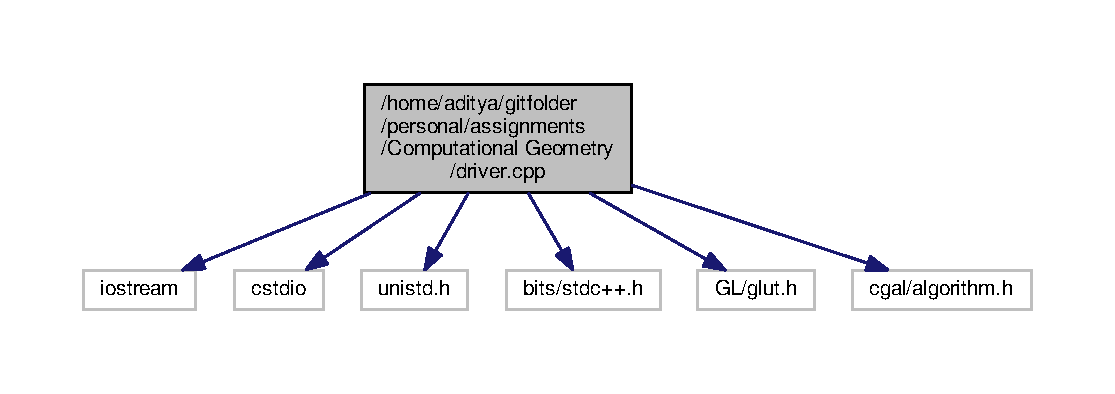
\includegraphics[width=350pt]{driver_8cpp__incl}
\end{center}
\end{figure}
\subsection*{Functions}
\begin{DoxyCompactItemize}
\item 
\hypertarget{driver_8cpp_a91c42686f3245f22fb6b17ba5372d92c}{}void \hyperlink{driver_8cpp_a91c42686f3245f22fb6b17ba5372d92c}{render\+Scene} ()\label{driver_8cpp_a91c42686f3245f22fb6b17ba5372d92c}

\begin{DoxyCompactList}\small\item\em Registered call back for G\+L display function. \end{DoxyCompactList}\item 
int \hyperlink{driver_8cpp_a0ddf1224851353fc92bfbff6f499fa97}{main} (int argc, char $\ast$argv\mbox{[}$\,$\mbox{]})
\begin{DoxyCompactList}\small\item\em Main function. \end{DoxyCompactList}\end{DoxyCompactItemize}


\subsection{Detailed Description}
Driver program that makes calls to Covex Hull A\+P\+I. 



\subsection{Function Documentation}
\hypertarget{driver_8cpp_a0ddf1224851353fc92bfbff6f499fa97}{}\index{driver.\+cpp@{driver.\+cpp}!main@{main}}
\index{main@{main}!driver.\+cpp@{driver.\+cpp}}
\subsubsection[{main}]{\setlength{\rightskip}{0pt plus 5cm}int main (
\begin{DoxyParamCaption}
\item[{int}]{argc, }
\item[{char $\ast$}]{argv\mbox{[}$\,$\mbox{]}}
\end{DoxyParamCaption}
)}\label{driver_8cpp_a0ddf1224851353fc92bfbff6f499fa97}


Main function. 


\begin{DoxyParams}{Parameters}
{\em argc} & default commandline argument. \\
\hline
{\em argv} & default commandline arguments. \\
\hline
\end{DoxyParams}

\begin{DoxyCode}
44 \{
45 
46     cin >> size >> animtog;
47     \textcolor{keywordflow}{for} ( \textcolor{keywordtype}{int} i = 0; i < size; i++ )
48     \{
49         \textcolor{keywordtype}{double} x, y;
50         cin >> x >> y;
51         S.addPoint( coord(x, y) );
52     \}
53 
54     glutInit(&argc, argv);
55     graphicsInitialize();
56     glutDisplayFunc( \hyperlink{driver_8cpp_a91c42686f3245f22fb6b17ba5372d92c}{renderScene} );
57     glutMainLoop();
58 
59     \textcolor{keywordflow}{return} 0;
60 \}
\end{DoxyCode}

\hypertarget{driver3_8cpp}{}\section{/home/aditya/gitfolder/personal/assignments/\+Computational Geometry/driver3.cpp File Reference}
\label{driver3_8cpp}\index{/home/aditya/gitfolder/personal/assignments/\+Computational Geometry/driver3.\+cpp@{/home/aditya/gitfolder/personal/assignments/\+Computational Geometry/driver3.\+cpp}}


Driver file to execute the 1 D Range Query on a set of data points. It calls the function to determine the convex hull which are implemented in algorithm.\+h file. It includes iostream, math.\+h, string, set, cstring, vector, fstream, sstream, cstdlib, algorithm,locale header files and bbst.\+h header file.  


{\ttfamily \#include $<$iostream$>$}\\*
{\ttfamily \#include $<$math.\+h$>$}\\*
{\ttfamily \#include $<$string$>$}\\*
{\ttfamily \#include $<$set$>$}\\*
{\ttfamily \#include $<$cstring$>$}\\*
{\ttfamily \#include $<$vector$>$}\\*
{\ttfamily \#include $<$fstream$>$}\\*
{\ttfamily \#include $<$sstream$>$}\\*
{\ttfamily \#include $<$cstdlib$>$}\\*
{\ttfamily \#include $<$algorithm$>$}\\*
{\ttfamily \#include $<$locale$>$}\\*
{\ttfamily \#include $<$ctime$>$}\\*
{\ttfamily \#include \char`\"{}temp/data/bbst.\+h\char`\"{}}\\*
Include dependency graph for driver3.\+cpp\+:\nopagebreak
\begin{figure}[H]
\begin{center}
\leavevmode
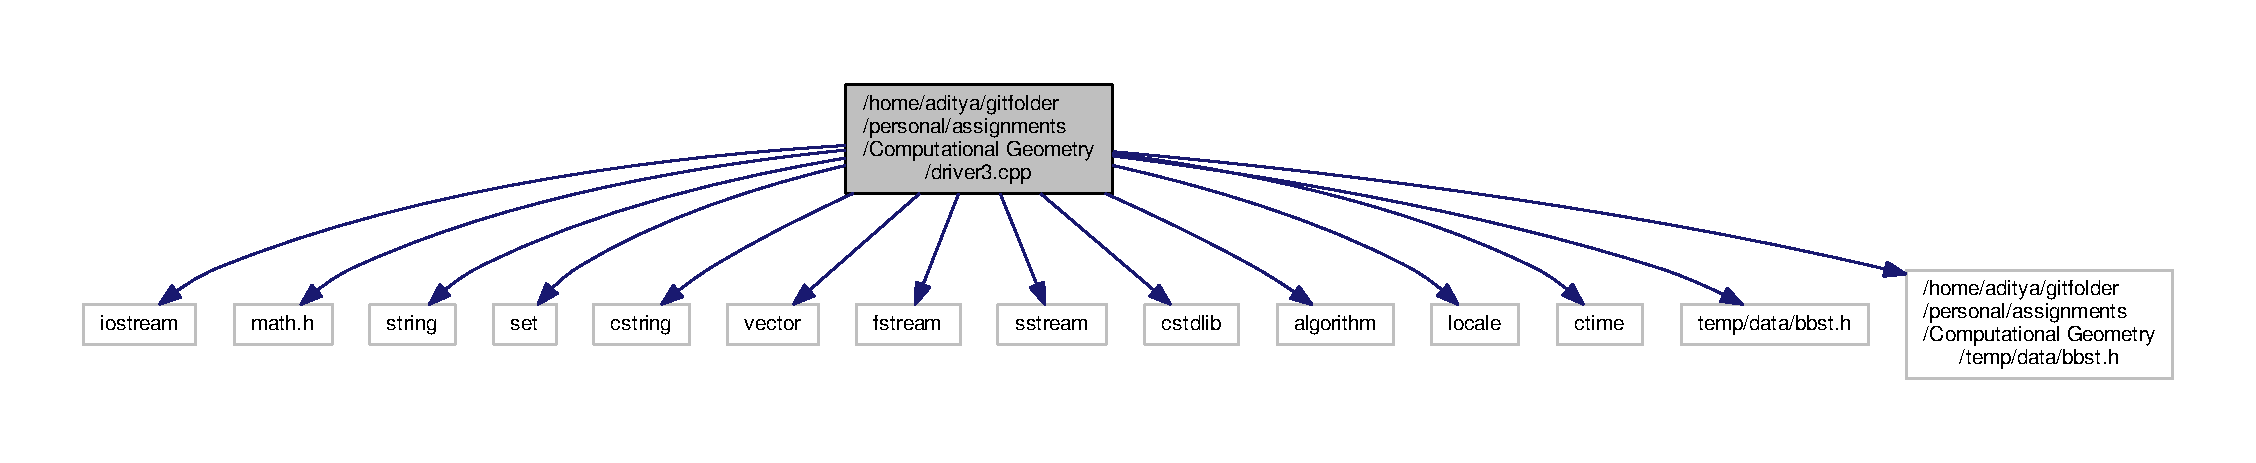
\includegraphics[width=350pt]{driver3_8cpp__incl}
\end{center}
\end{figure}
\subsection*{Functions}
\begin{DoxyCompactItemize}
\item 
\hypertarget{driver3_8cpp_ae66f6b31b5ad750f1fe042a706a4e3d4}{}int {\bfseries main} ()\label{driver3_8cpp_ae66f6b31b5ad750f1fe042a706a4e3d4}

\end{DoxyCompactItemize}


\subsection{Detailed Description}
Driver file to execute the 1 D Range Query on a set of data points. It calls the function to determine the convex hull which are implemented in algorithm.\+h file. It includes iostream, math.\+h, string, set, cstring, vector, fstream, sstream, cstdlib, algorithm,locale header files and bbst.\+h header file. 


\hypertarget{generator_8cpp}{}\section{/home/aditya/gitfolder/personal/assignments/\+Computational Geometry/generator.cpp File Reference}
\label{generator_8cpp}\index{/home/aditya/gitfolder/personal/assignments/\+Computational Geometry/generator.\+cpp@{/home/aditya/gitfolder/personal/assignments/\+Computational Geometry/generator.\+cpp}}


Generates random dataset from a specified distribution.  


{\ttfamily \#include $<$stdlib.\+h$>$}\\*
{\ttfamily \#include $<$stdio.\+h$>$}\\*
{\ttfamily \#include $<$iostream$>$}\\*
{\ttfamily \#include $<$random$>$}\\*
{\ttfamily \#include $<$bits/stdc++.\+h$>$}\\*
Include dependency graph for generator.\+cpp\+:\nopagebreak
\begin{figure}[H]
\begin{center}
\leavevmode
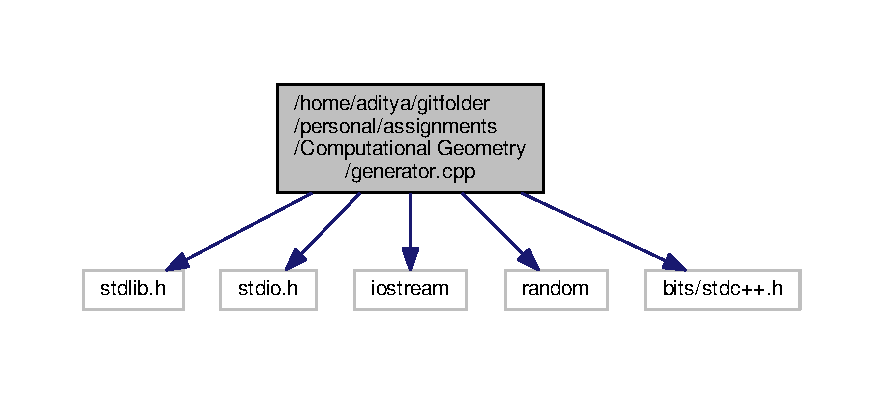
\includegraphics[width=350pt]{generator_8cpp__incl}
\end{center}
\end{figure}
\subsection*{Functions}
\begin{DoxyCompactItemize}
\item 
\hypertarget{generator_8cpp_ae66f6b31b5ad750f1fe042a706a4e3d4}{}int {\bfseries main} ()\label{generator_8cpp_ae66f6b31b5ad750f1fe042a706a4e3d4}

\end{DoxyCompactItemize}


\subsection{Detailed Description}
Generates random dataset from a specified distribution. 


%--- End generated contents ---

% Index
\backmatter
\newpage
\phantomsection
\clearemptydoublepage
\addcontentsline{toc}{chapter}{Index}
\printindex

\end{document}
